\chapter{Sequence Modeling}
%Authors: Sarthak Agarwal, Raghav Jajodia, Ieshan Vaidya
%2019-03-31
In this chapter two applications of sequential networks are present:
\begin{enumerate}
    \item Sequence Classification - Given character sequences, classify them into pre-specified categories.
    \item Signal Echoing - Given an input signal, generate the same signal but with a lag of $n$ steps.
\end{enumerate}
Both of these tasks test the capability of the network to keep track of arbitrary long-term dependencies in the input sequences.

\section{Sequence Classification}
\label{sec:SeqClassification}
%Authors: Ieshan Vaidya
%2019-03-31
To illustrate the necessity of long-term memory, consider a sequence classification problem. 
Each input sequence starts with the letter B and ends with E (the trigger symbol). 
The symbols in-between are randomly chosen from the set \{a, b, c, d\} except for two elements at positions $t_1$ and $t_2$ that are either X or Y. 
The classification targets are 4 sequence classes Q, R, S and U which depend on the temporal order of X and Y. 
The rules are
\begin{align*}
    \text{X, X} &\rightarrow \text{Q} \\
    \text{X, Y} &\rightarrow \text{R} \\
    \text{Y, X} &\rightarrow \text{S} \\
    \text{Y, Y} &\rightarrow \text{U}
\end{align*}
There are 5 difficulty levels for this problem -
\begin{enumerate}
    \item EASY : The length of the sequence is randomly chosen from [7, 8]; $t_1$ is randomly chosen from [1, 2]; $t_2$ is randomly chosen from [4, 5].
    \item NORMAL : The length of the sequence is randomly chosen from [30, 40]; $t_1$ is randomly chosen from [2, 5]; $t_2$ is randomly chosen from [20, 27].
    \item MODERATE : The length of the sequence is randomly chosen from [60, 80]; $t_1$ is randomly chosen from [10, 20]; $t_2$ is randomly chosen from [45, 54].
    \item HARD : The length of the sequence is randomly chosen from [100, 110]; $t_1$ is randomly chosen from [10, 20]; $t_2$ is randomly chosen from [50, 60].
    \item NIGHTMARE : The length of the sequence is randomly chosen from [300, 500]; $t_1$ is randomly chosen from [10, 80]; $t_2$ is randomly chosen from [250, 290].
\end{enumerate}
As one can see, long-term memory of X or Y symbols is required to correctly classify the sequence. 
The HARD difficulty is identical to the original setting of \cite{article-lstm}.
In the subsequent sections, we will explore the data and train two models. 
Full details of implementation can be found at \href{https://github.com/Atcold/pytorch-Deep-Learning-Minicourse/blob/master/08-seq_classification.ipynb}{Sequence Classification}.

\subsection{Dataset Exploration}
%Authors: Ieshan Vaidya
%2019-03-31
Consider sequences of EASY difficulty generated using \texttt{get\_predefined\_generator} method of the \texttt{TemporalOrderExp6aSequence} class.
\begin{minted}[breaklines]{python}
from sequential_tasks import TemporalOrderExp6aSequence

# Create a data generator.
example_generator = TemporalOrderExp6aSequence.get_predefined_generator(
    # The first argument is the difficulty level of the classification task.
    difficulty_level=TemporalOrderExp6aSequence.DifficultyLevel.EASY,
    # The second argument is the number of sequences generated in each batch of data.
    batch_size=32,
)
\end{minted}
Let's print the details of a sample.
\begin{verbatim}
The return type is a <class 'tuple'> with length 2.
The first item in the tuple is the batch of sequences with shape (32, 9, 8).
The first element in the batch of sequences is:
 [[0 0 0 0 0 0 0 0]
 [0 0 0 0 0 0 1 0]
 [0 0 0 1 0 0 0 0]
 [1 0 0 0 0 0 0 0]
 [0 0 0 0 1 0 0 0]
 [1 0 0 0 0 0 0 0]
 [0 0 0 0 1 0 0 0]
 [0 0 0 1 0 0 0 0]
 [0 0 0 0 0 0 0 1]]
The second item in the tuple is the corresponding batch of class labels with shape (32, 4).
The first element in the batch of class labels is:
 [1. 0. 0. 0.]
\end{verbatim}
As observed in the output, the sequences are 1-hot encoded in memory. Since there are 8 possible symbols \{X, Y, a, b, c, d, B, E\}, the last dimension has size 8. 
The first dimension is the batch size whereas the second dimension corresponds to the length of the sequence. 
Since length of the sequence is variable, to maintain consistency, the data is zero-padded at the beginning. 
Zero-padding is performed at the beginning rather than the end so that back-propagation can be terminated at the start trigger (B).

\begin{minted}[breaklines]{python}
# Decoding the first sequence.
sequence_decoded = example_generator.decode_x(example_batch[0][0, :, :])

# Decoding the class label of the first sequence.
class_label_decoded = example_generator.decode_y(example_batch[1][0])
\end{minted}
The decoded sequence is given below.
\begin{verbatim}
The sequence is: BbXcXcbE
The class label is: Q
\end{verbatim}

\subsection{Model Definition}
%Authors: Ieshan Vaidya
%2019-03-31
Let's define two models to capture memory - RNN and LSTM. 
\begin{minted}[breaklines]{python}
import torch
import torch.nn as nn

# Set the random seed for reproducible results.
torch.manual_seed(1)

class SimpleRNN(nn.Module):
    def __init__(self, input_size, hidden_size, output_size):
        # This just calls the base class constructor.
        super().__init__()
        # Neural network layers assigned as attributes of a Module subclass
        # have their parameters registered for training automatically.
        self.rnn = torch.nn.RNN(input_size, hidden_size, nonlinearity='relu', batch_first=True)
        self.linear = torch.nn.Linear(hidden_size, output_size)

    def forward(self, x):
        # The RNN also returns its hidden state but we don't use it.
        # While the RNN can also take a hidden state as input, the RNN
        # gets passed a hidden state initialized with zeros by default.
        x, _ = self.rnn(x)
        x = self.linear(x)
        return x
    
class SimpleLSTM(nn.Module):
    def __init__(self, input_size, hidden_size, output_size):
        super().__init__()
        self.lstm = torch.nn.LSTM(input_size, hidden_size, batch_first=True)
        self.linear = torch.nn.Linear(hidden_size, output_size)

    def forward(self, x):
        x, _ = self.lstm(x)
        x = self.linear(x)
        return x
\end{minted}
The prediction is the argmax of the linear layer output.
During training, the loss used is Cross Entropy.

\subsection{Experiment 1 : EASY Difficulty}
%Authors: Ieshan Vaidya
%2019-03-31
Let's consider EASY difficulty first. Both the models are trained for 10 epochs. \cref{fig:rnn_easy_10} shows the RNN model performance.

\begin{minted}[breaklines]{python}
# Setup the training and test data generators.
difficulty     = TemporalOrderExp6aSequence.DifficultyLevel.EASY
batch_size     = 32
train_data_gen = TemporalOrderExp6aSequence.get_predefined_generator(difficulty, batch_size)
test_data_gen  = TemporalOrderExp6aSequence.get_predefined_generator(difficulty, batch_size)

# Setup the RNN and training settings.
input_size  = train_data_gen.n_symbols
hidden_size = 4
output_size = train_data_gen.n_classes
model       = SimpleRNN(input_size, hidden_size, output_size)
criterion   = torch.nn.CrossEntropyLoss()
optimizer   = torch.optim.RMSprop(model.parameters(), lr=0.001)
max_epochs  = 10

# Train the model.
model = train_and_test(model, train_data_gen, test_data_gen, criterion, optimizer, max_epochs)

for parameter_group in list(model.parameters()):
    print(parameter_group.size())
\end{minted}
\begin{figure}[H]
    \centering
    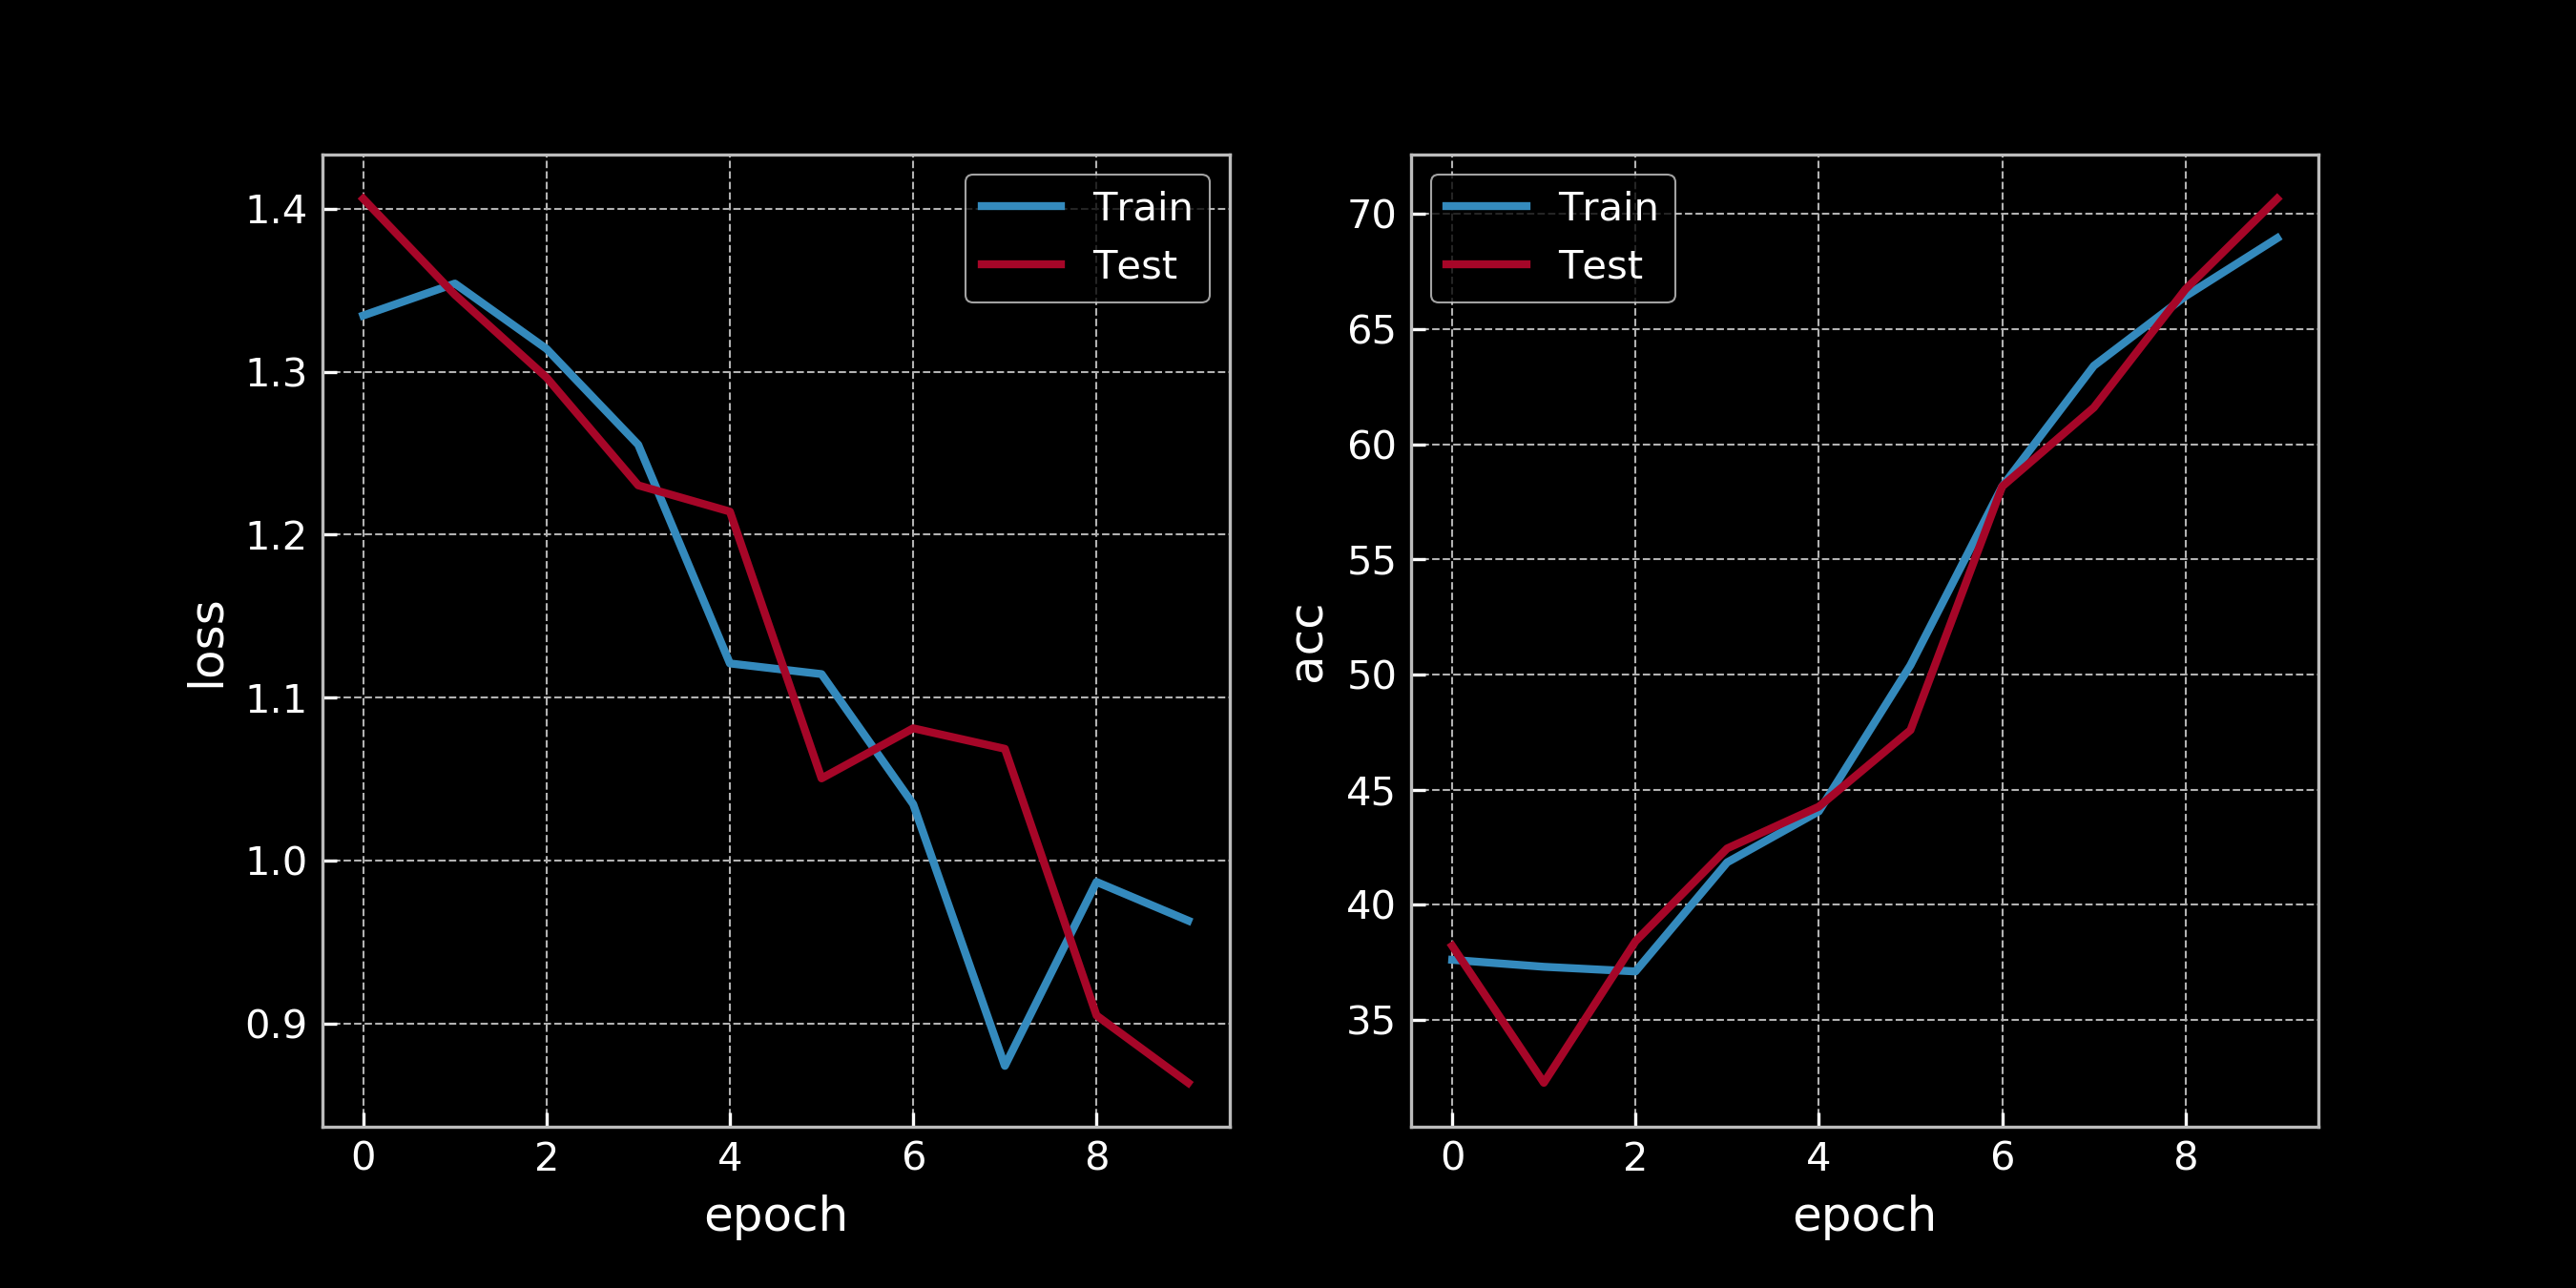
\includegraphics[width=0.5\linewidth]{labs/08/images/rnn_easy_10.png}
    \caption{EASY Difficulty - RNN Model for 10 epochs}
    \label{fig:rnn_easy_10}
\end{figure}

Using 10 epochs, we obtain $\approx 70\%$ in testing accuracy. 
We observe better testing accuracy than training accuracy during certain periods. 
The reason for this is that the training accuracy is computed with the model trained using the last batch whereas the testing accuracy is computed with the model trained using the current batch. 
One should instead compare the current training accuracy with the test accuracy one step back.
\cref{fig:lstm_easy_10} shows the performance of LSTM model.

\begin{figure}[H]
    \centering
    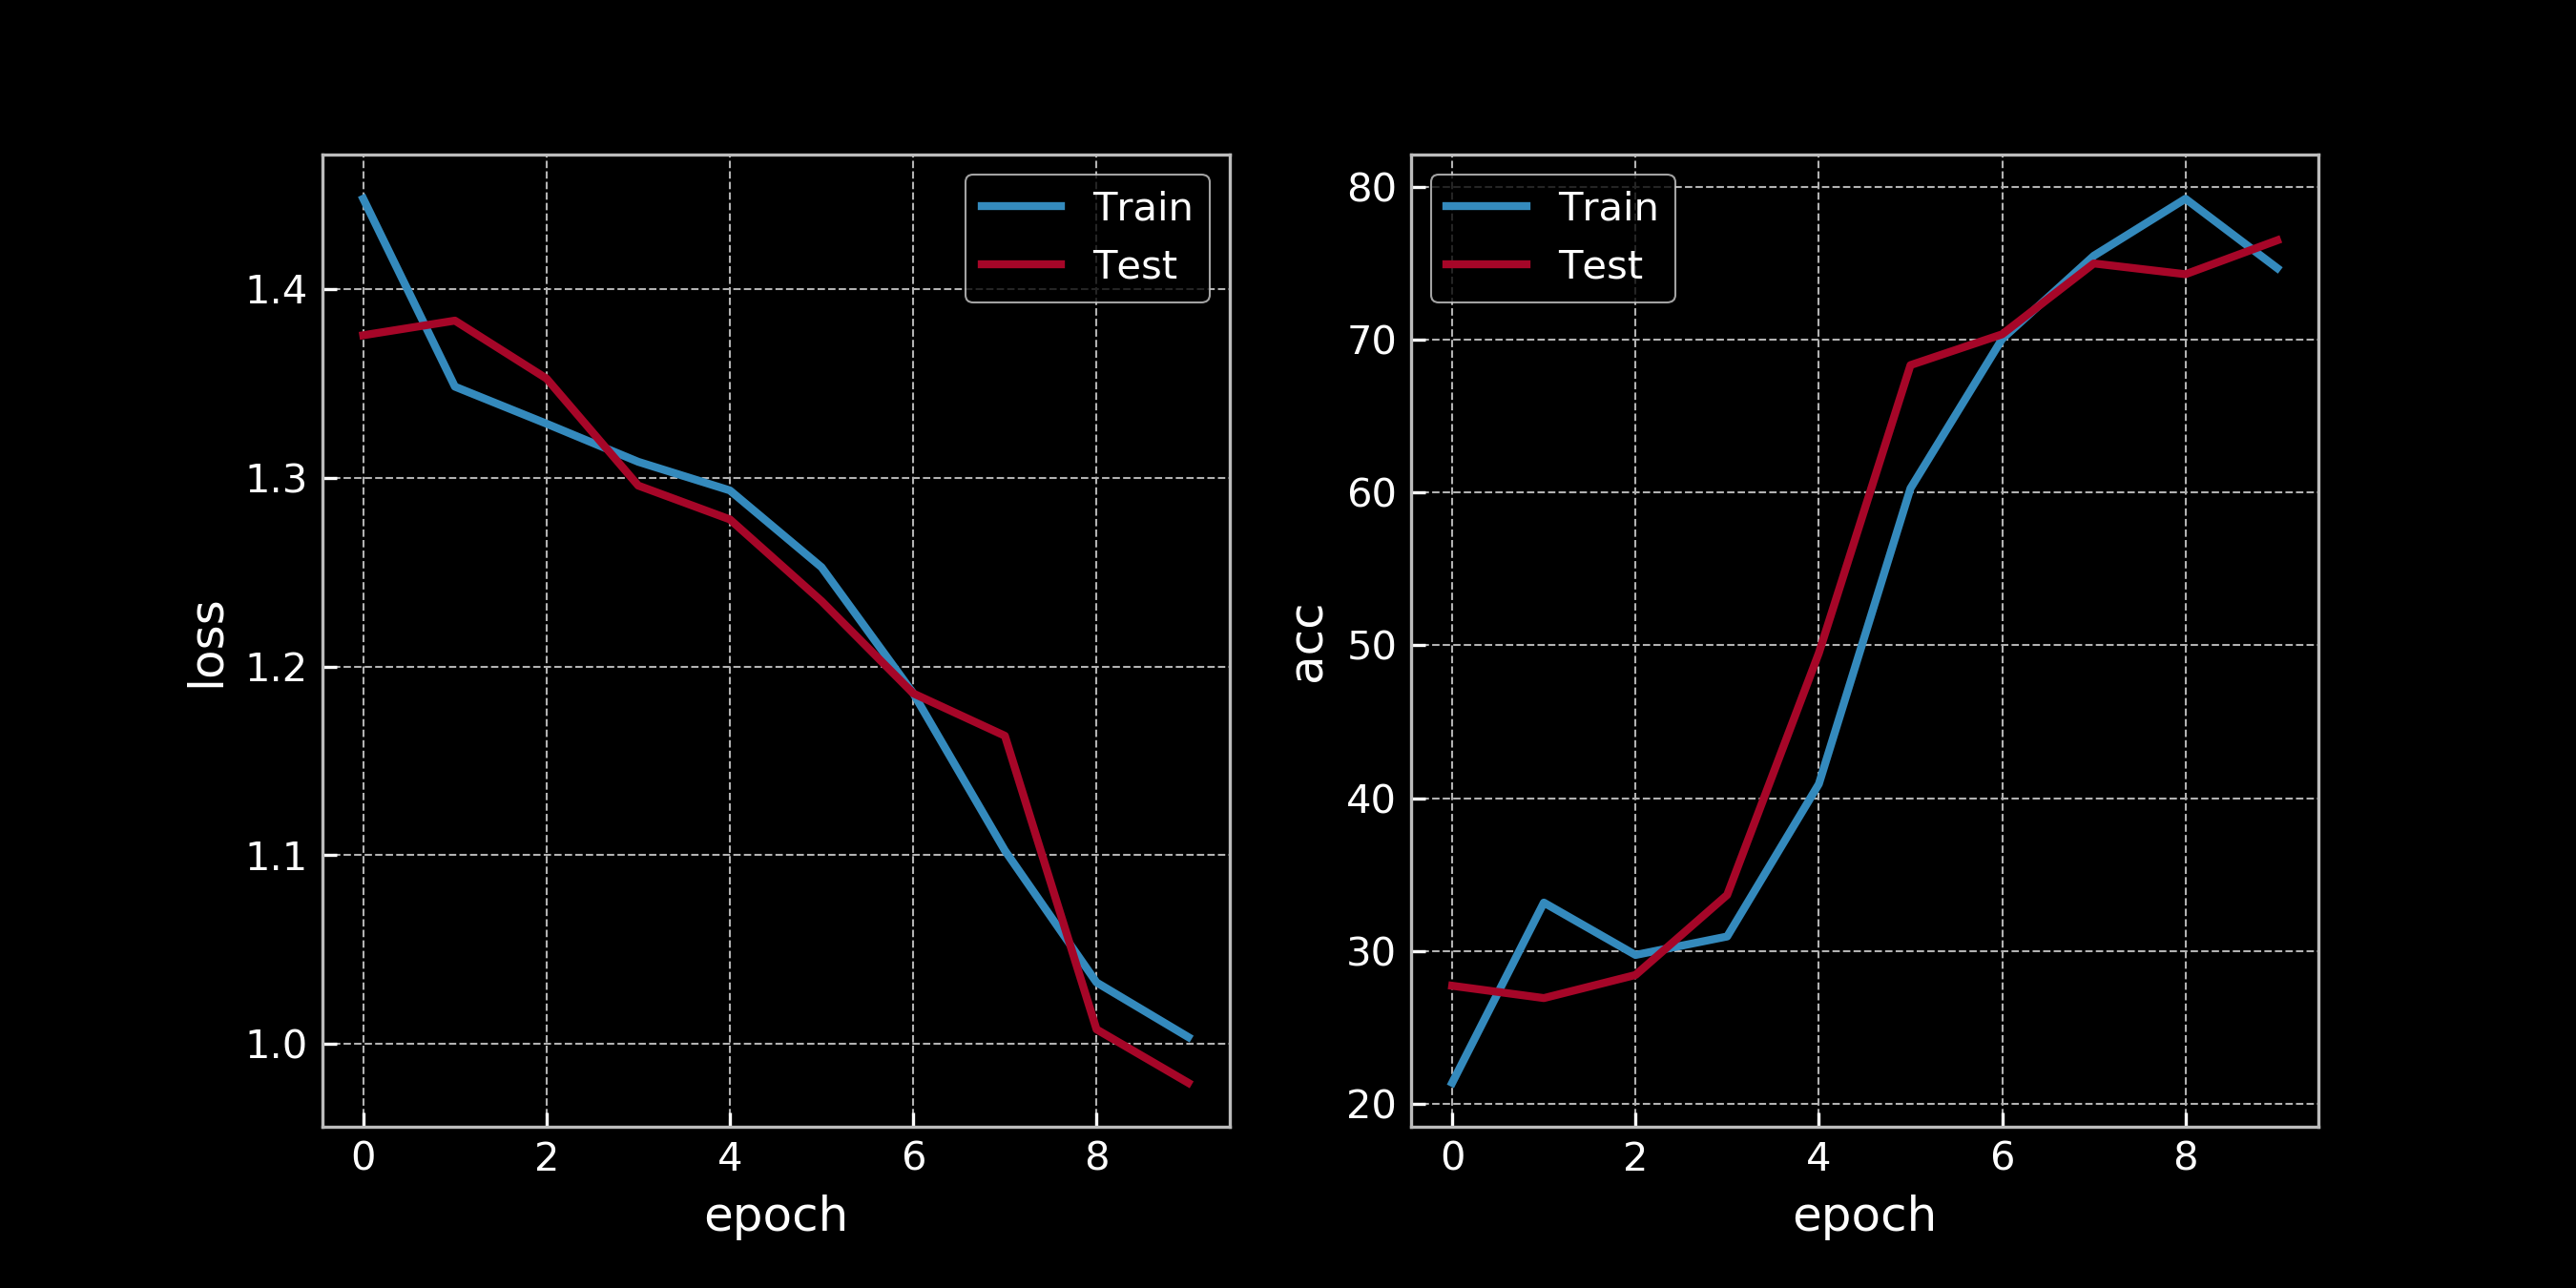
\includegraphics[width=0.5\linewidth]{labs/08/images/lstm_easy_10.png}
    \caption{EASY Difficulty - LSTM Model for 10 epochs}
    \label{fig:lstm_easy_10}
\end{figure}

Since there is scope for further improvement, the models are trained for 100 epochs. 
\cref{fig:rnn_easy_100} and \cref{fig:lstm_easy_100} show the performances of RNN and LSTM models respectively.

\begin{figure}[H]
    \centering
    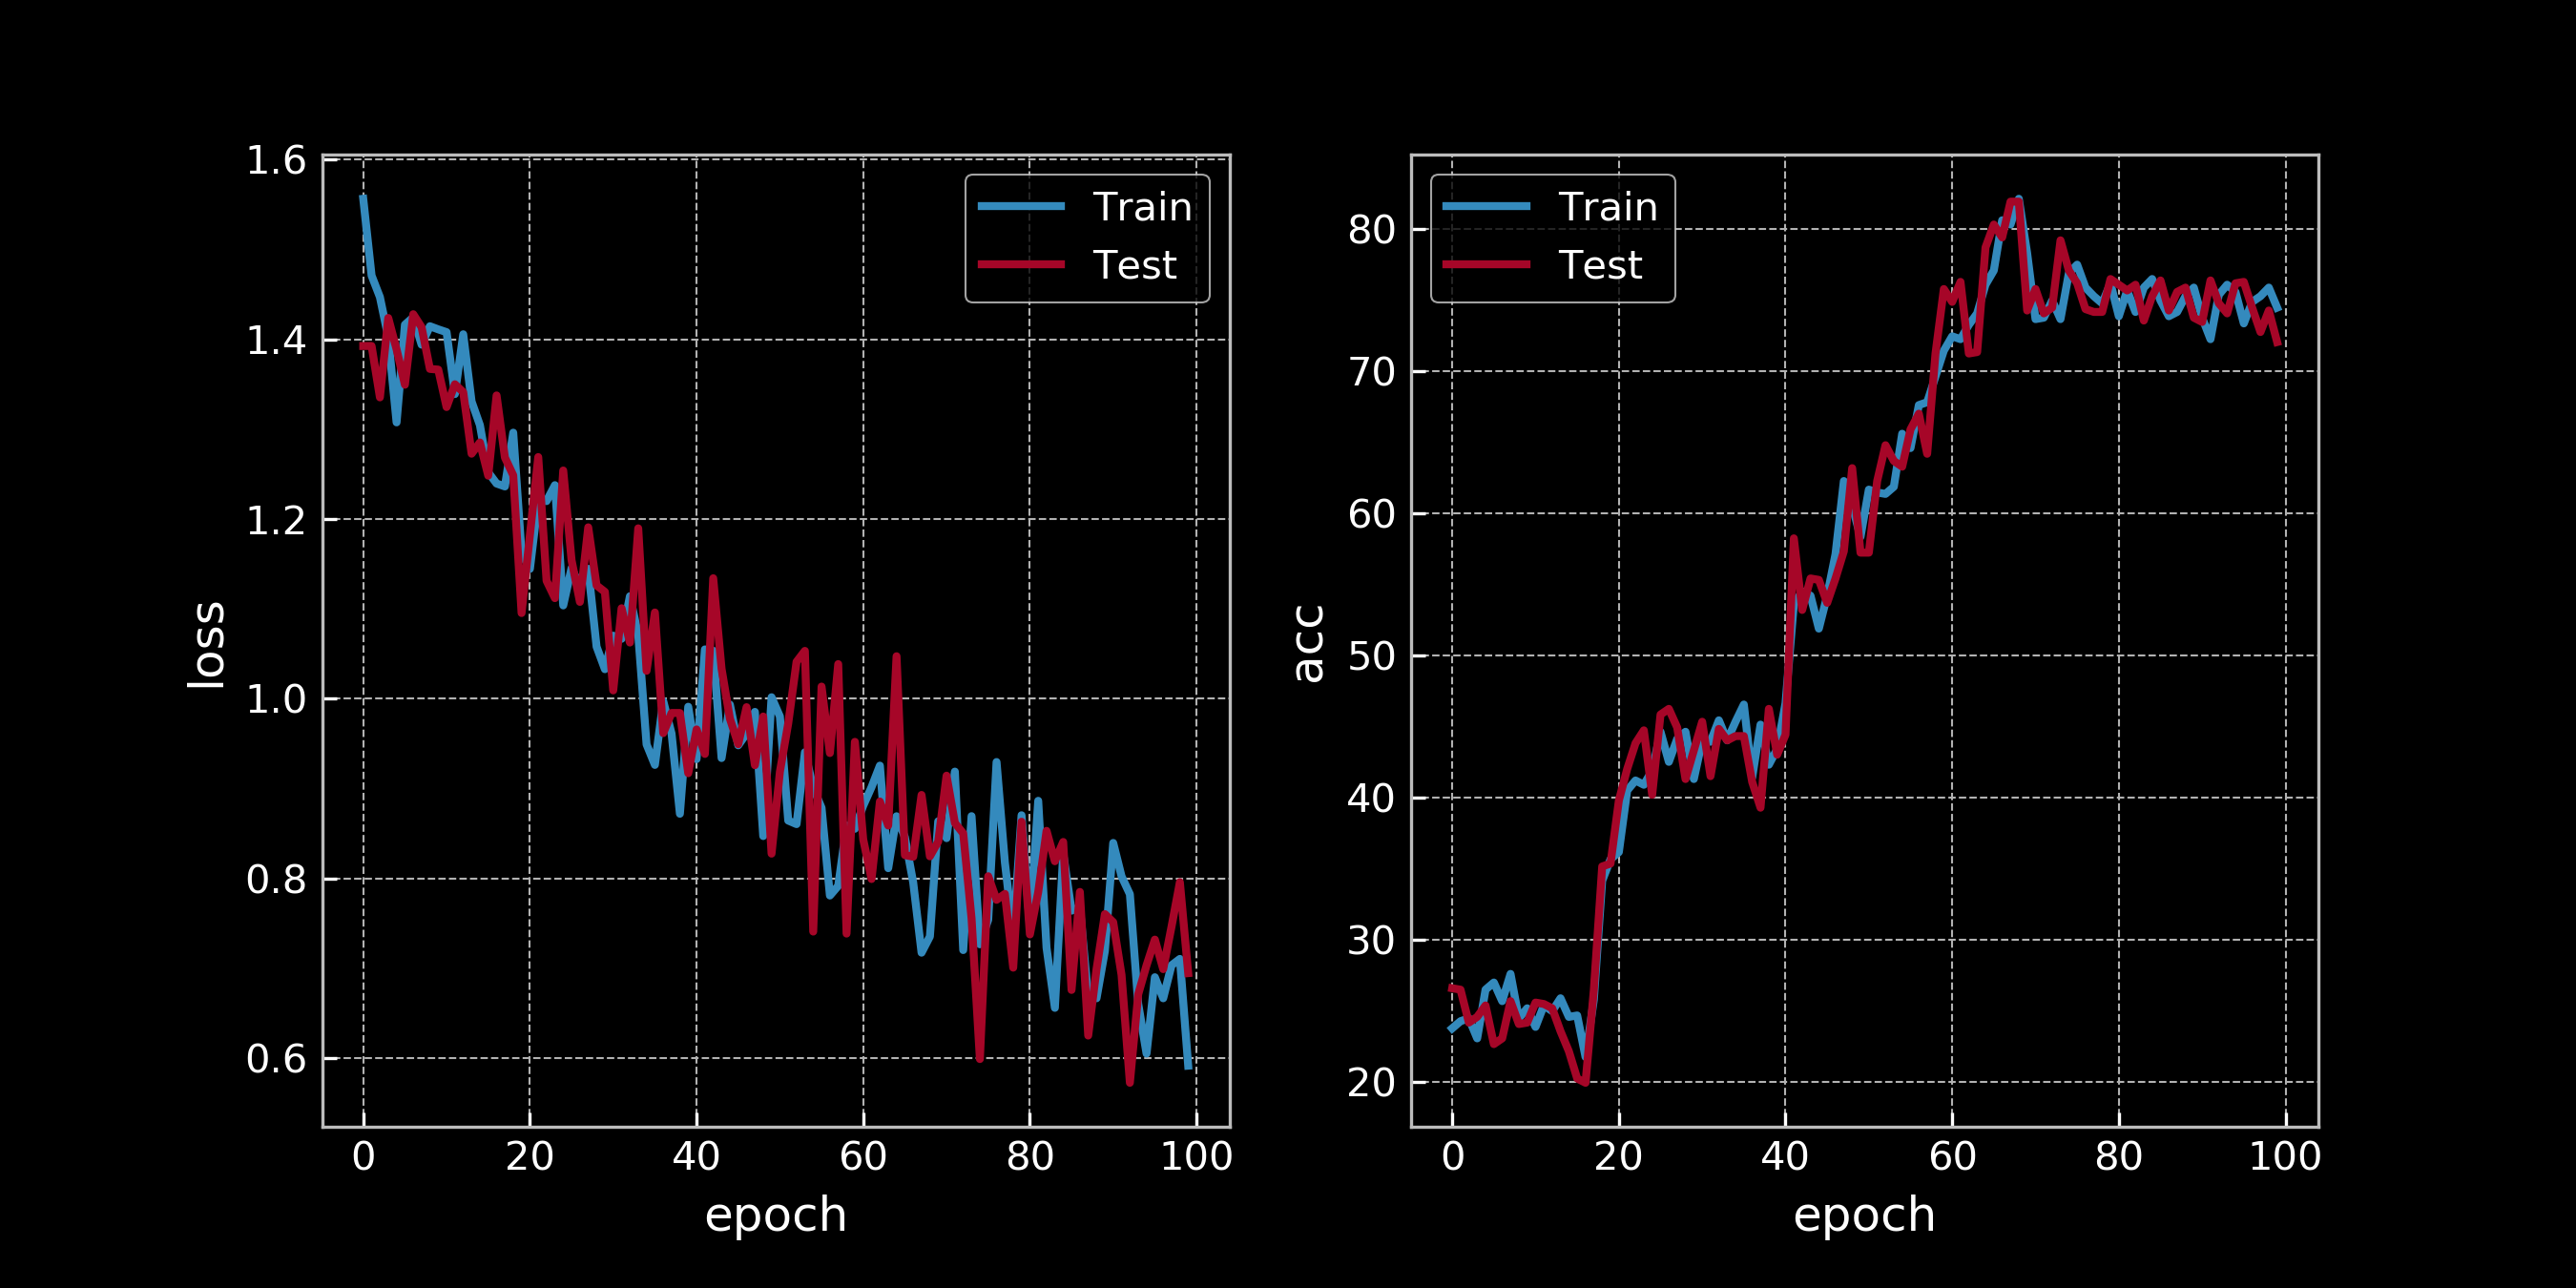
\includegraphics[width=0.5\linewidth]{labs/08/images/rnn_easy_100.png}
    \caption{EASY Difficulty - RNN Model for 100 epochs}
    \label{fig:rnn_easy_100}
\end{figure}

\begin{figure}[H]
    \centering
    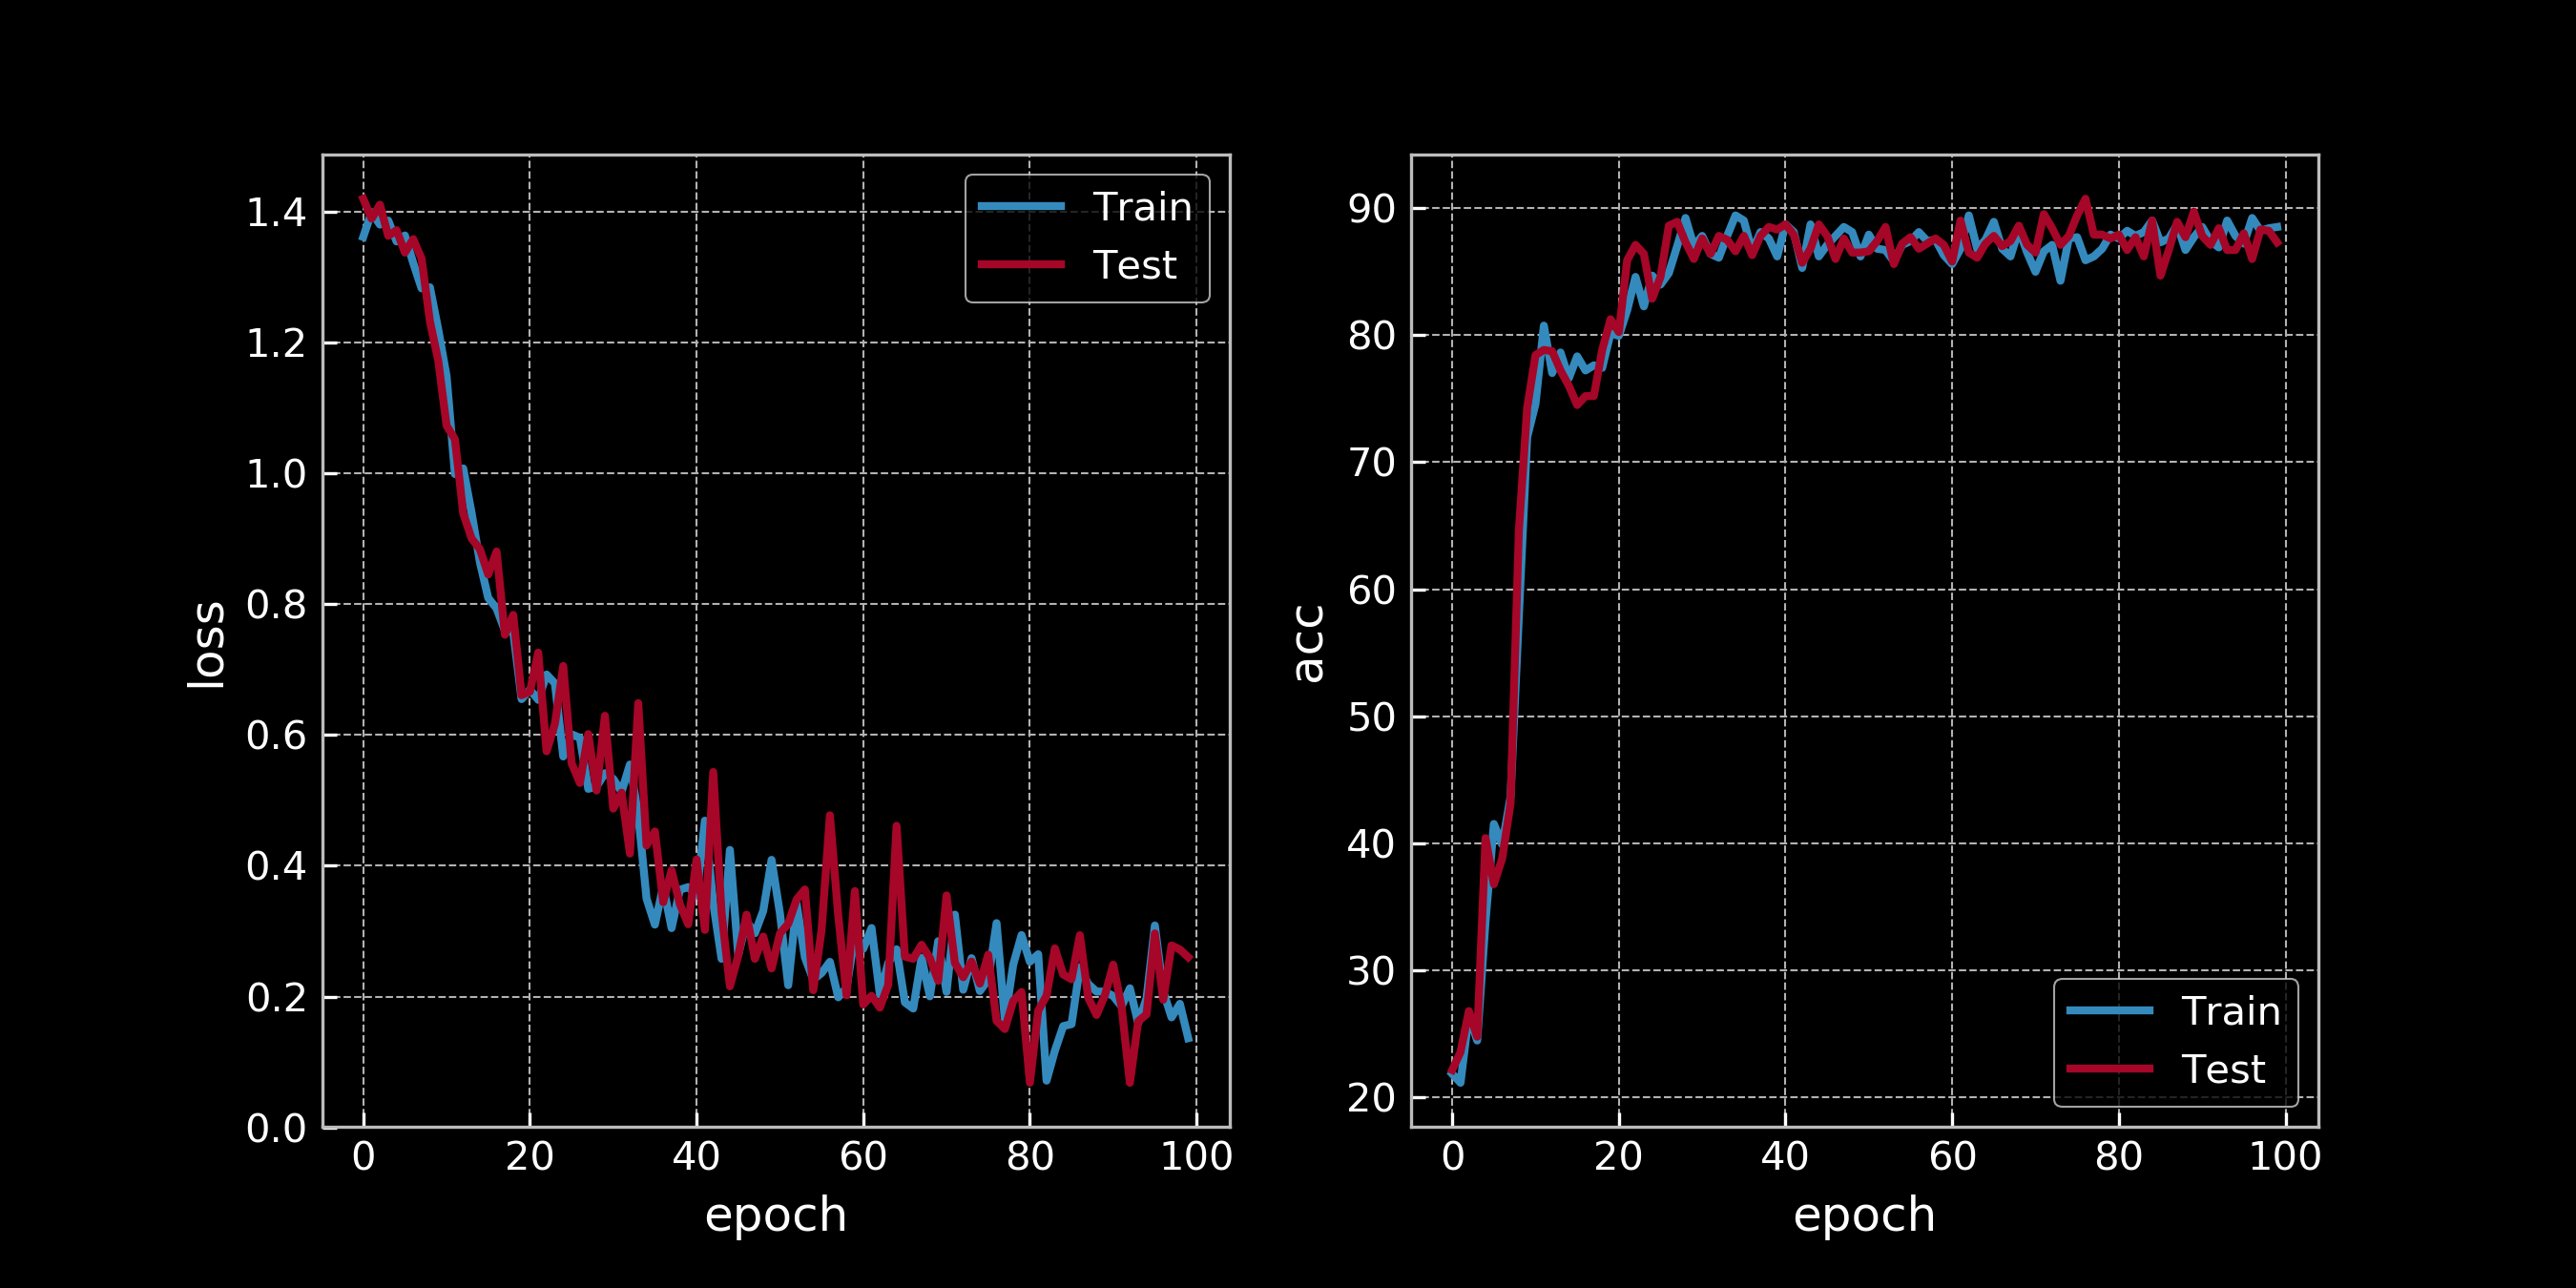
\includegraphics[width=0.5\linewidth]{labs/08/images/lstm_easy_100.png}
    \caption{EASY Difficulty - LSTM Model for 100 epochs}
    \label{fig:lstm_easy_100}
\end{figure}
Both models perform reasonably well and are able to memorize the correct class in EASY difficulty. 

\subsection{Experiment 2 : MODERATE Difficulty}
%Authors: Ieshan Vaidya
%2019-03-31
Now let's consider the MODERATE difficulty. The models are trained for 100 epochs and \cref{fig:rnn_moderate_100} and \cref{fig:lstm_moderate_100} show the performance of the RNN and LSTM models respectively.

\begin{figure}[H]
    \centering
    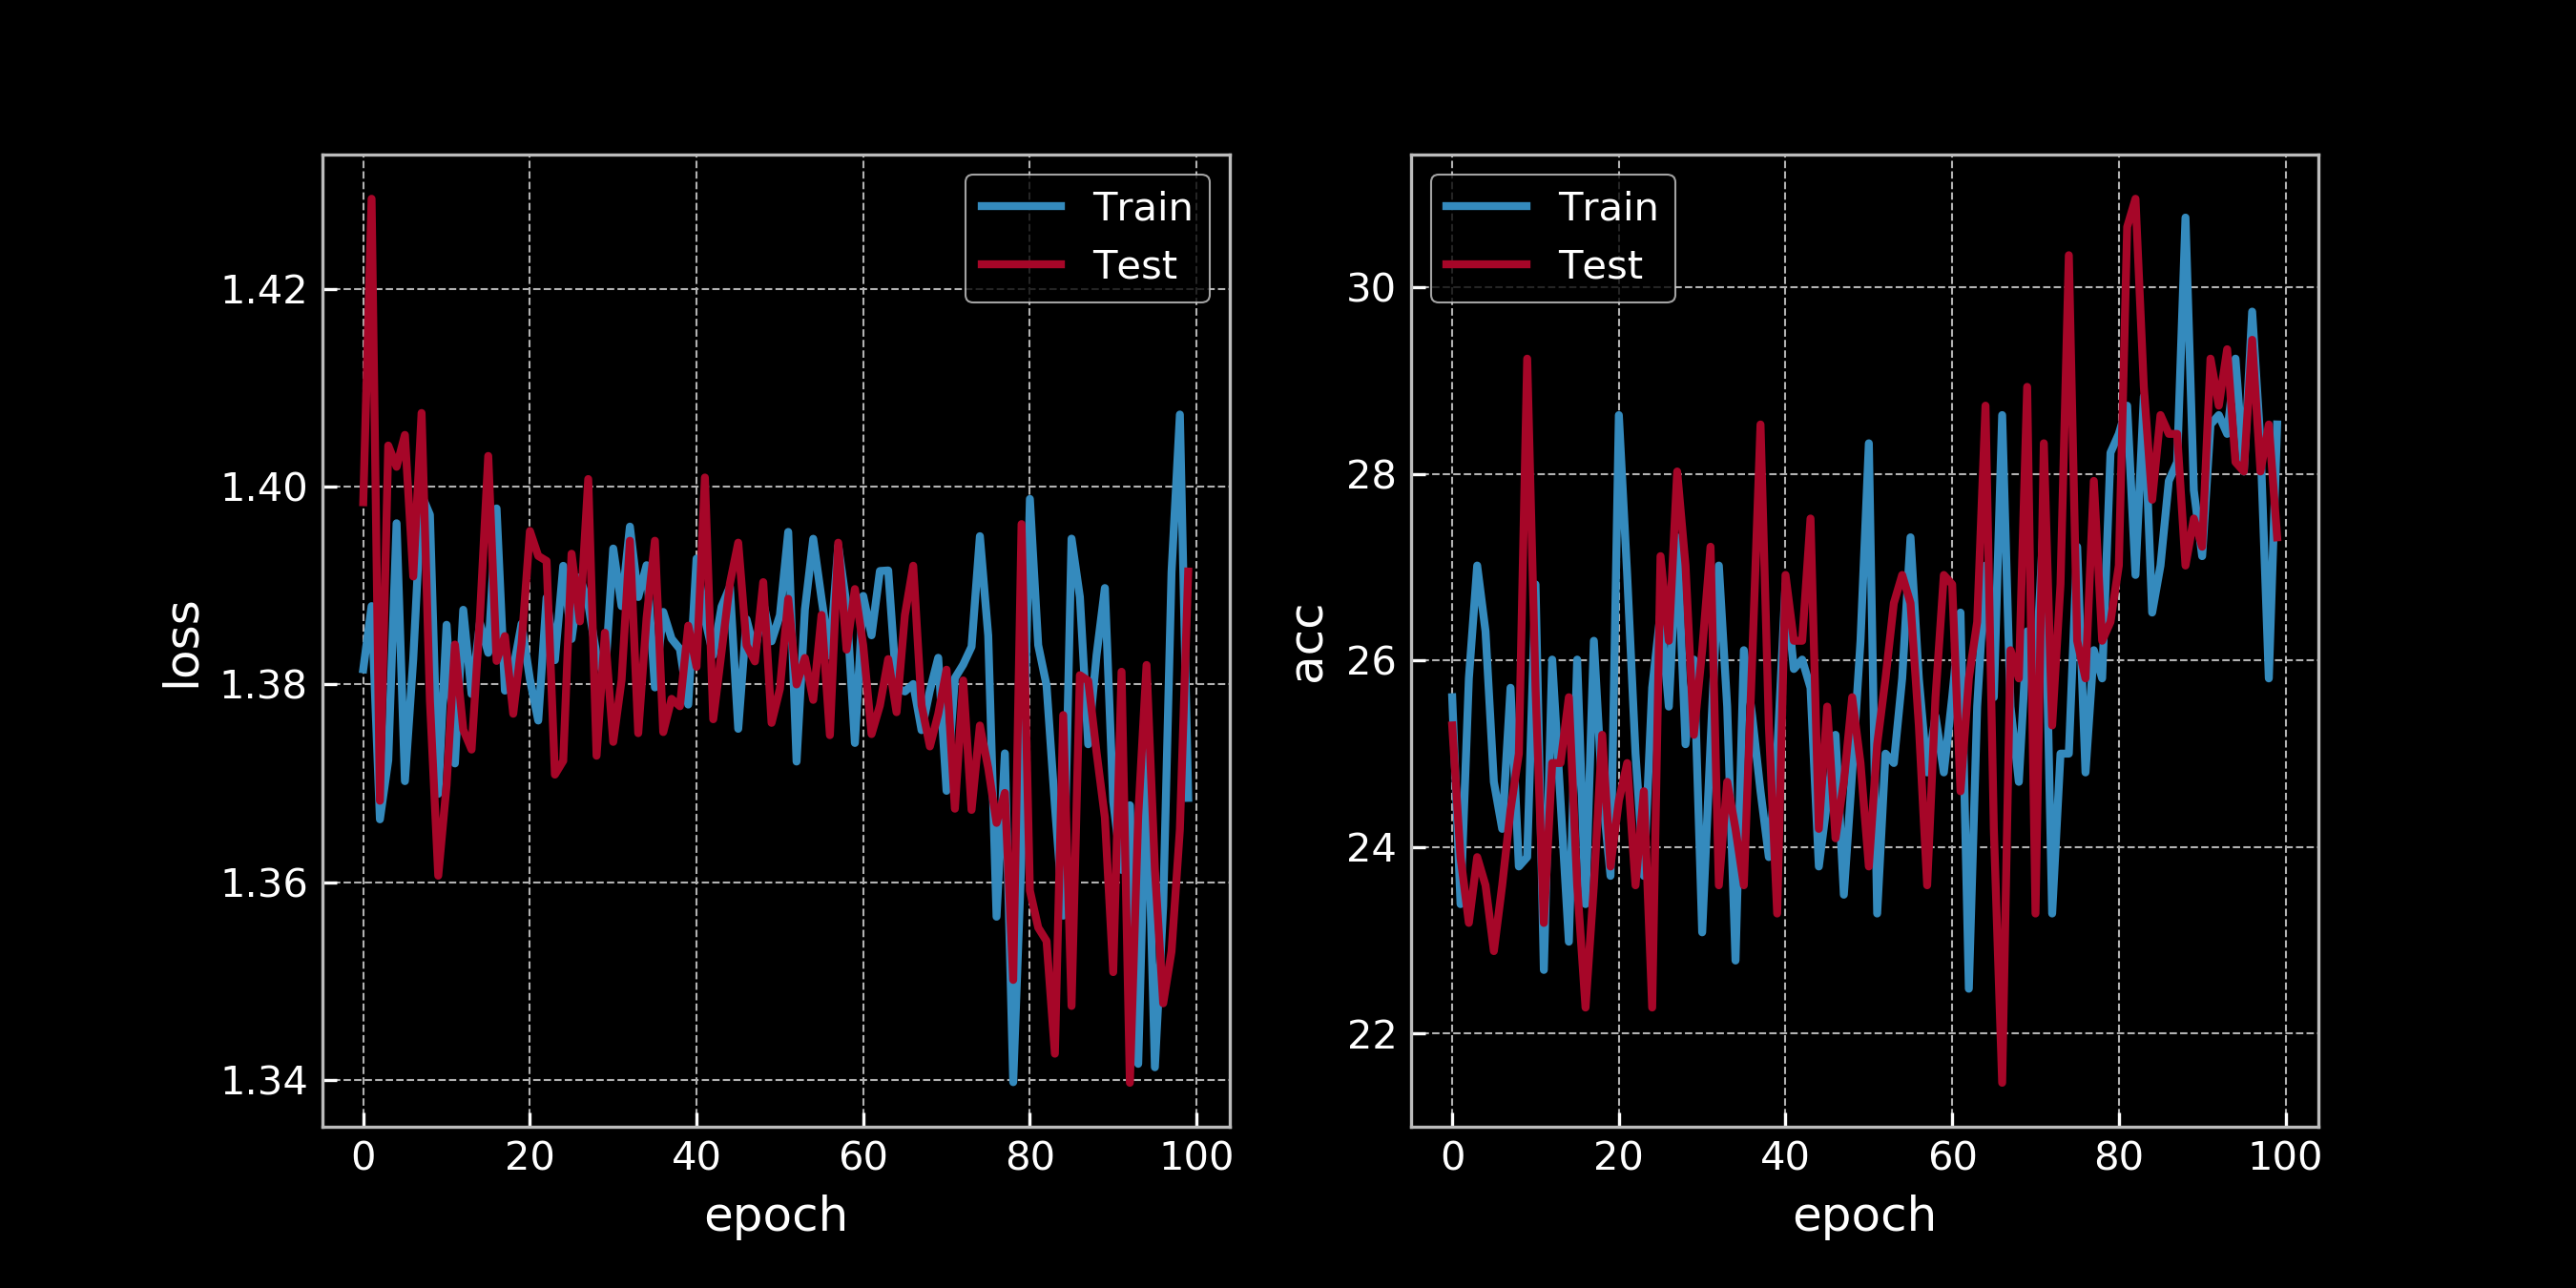
\includegraphics[width=0.5\linewidth]{labs/08/images/rnn_moderate_100.png}
    \caption{MODERATE Difficulty - RNN Model for 100 epochs}
    \label{fig:rnn_moderate_100}
\end{figure}

\begin{figure}[H]
    \centering
    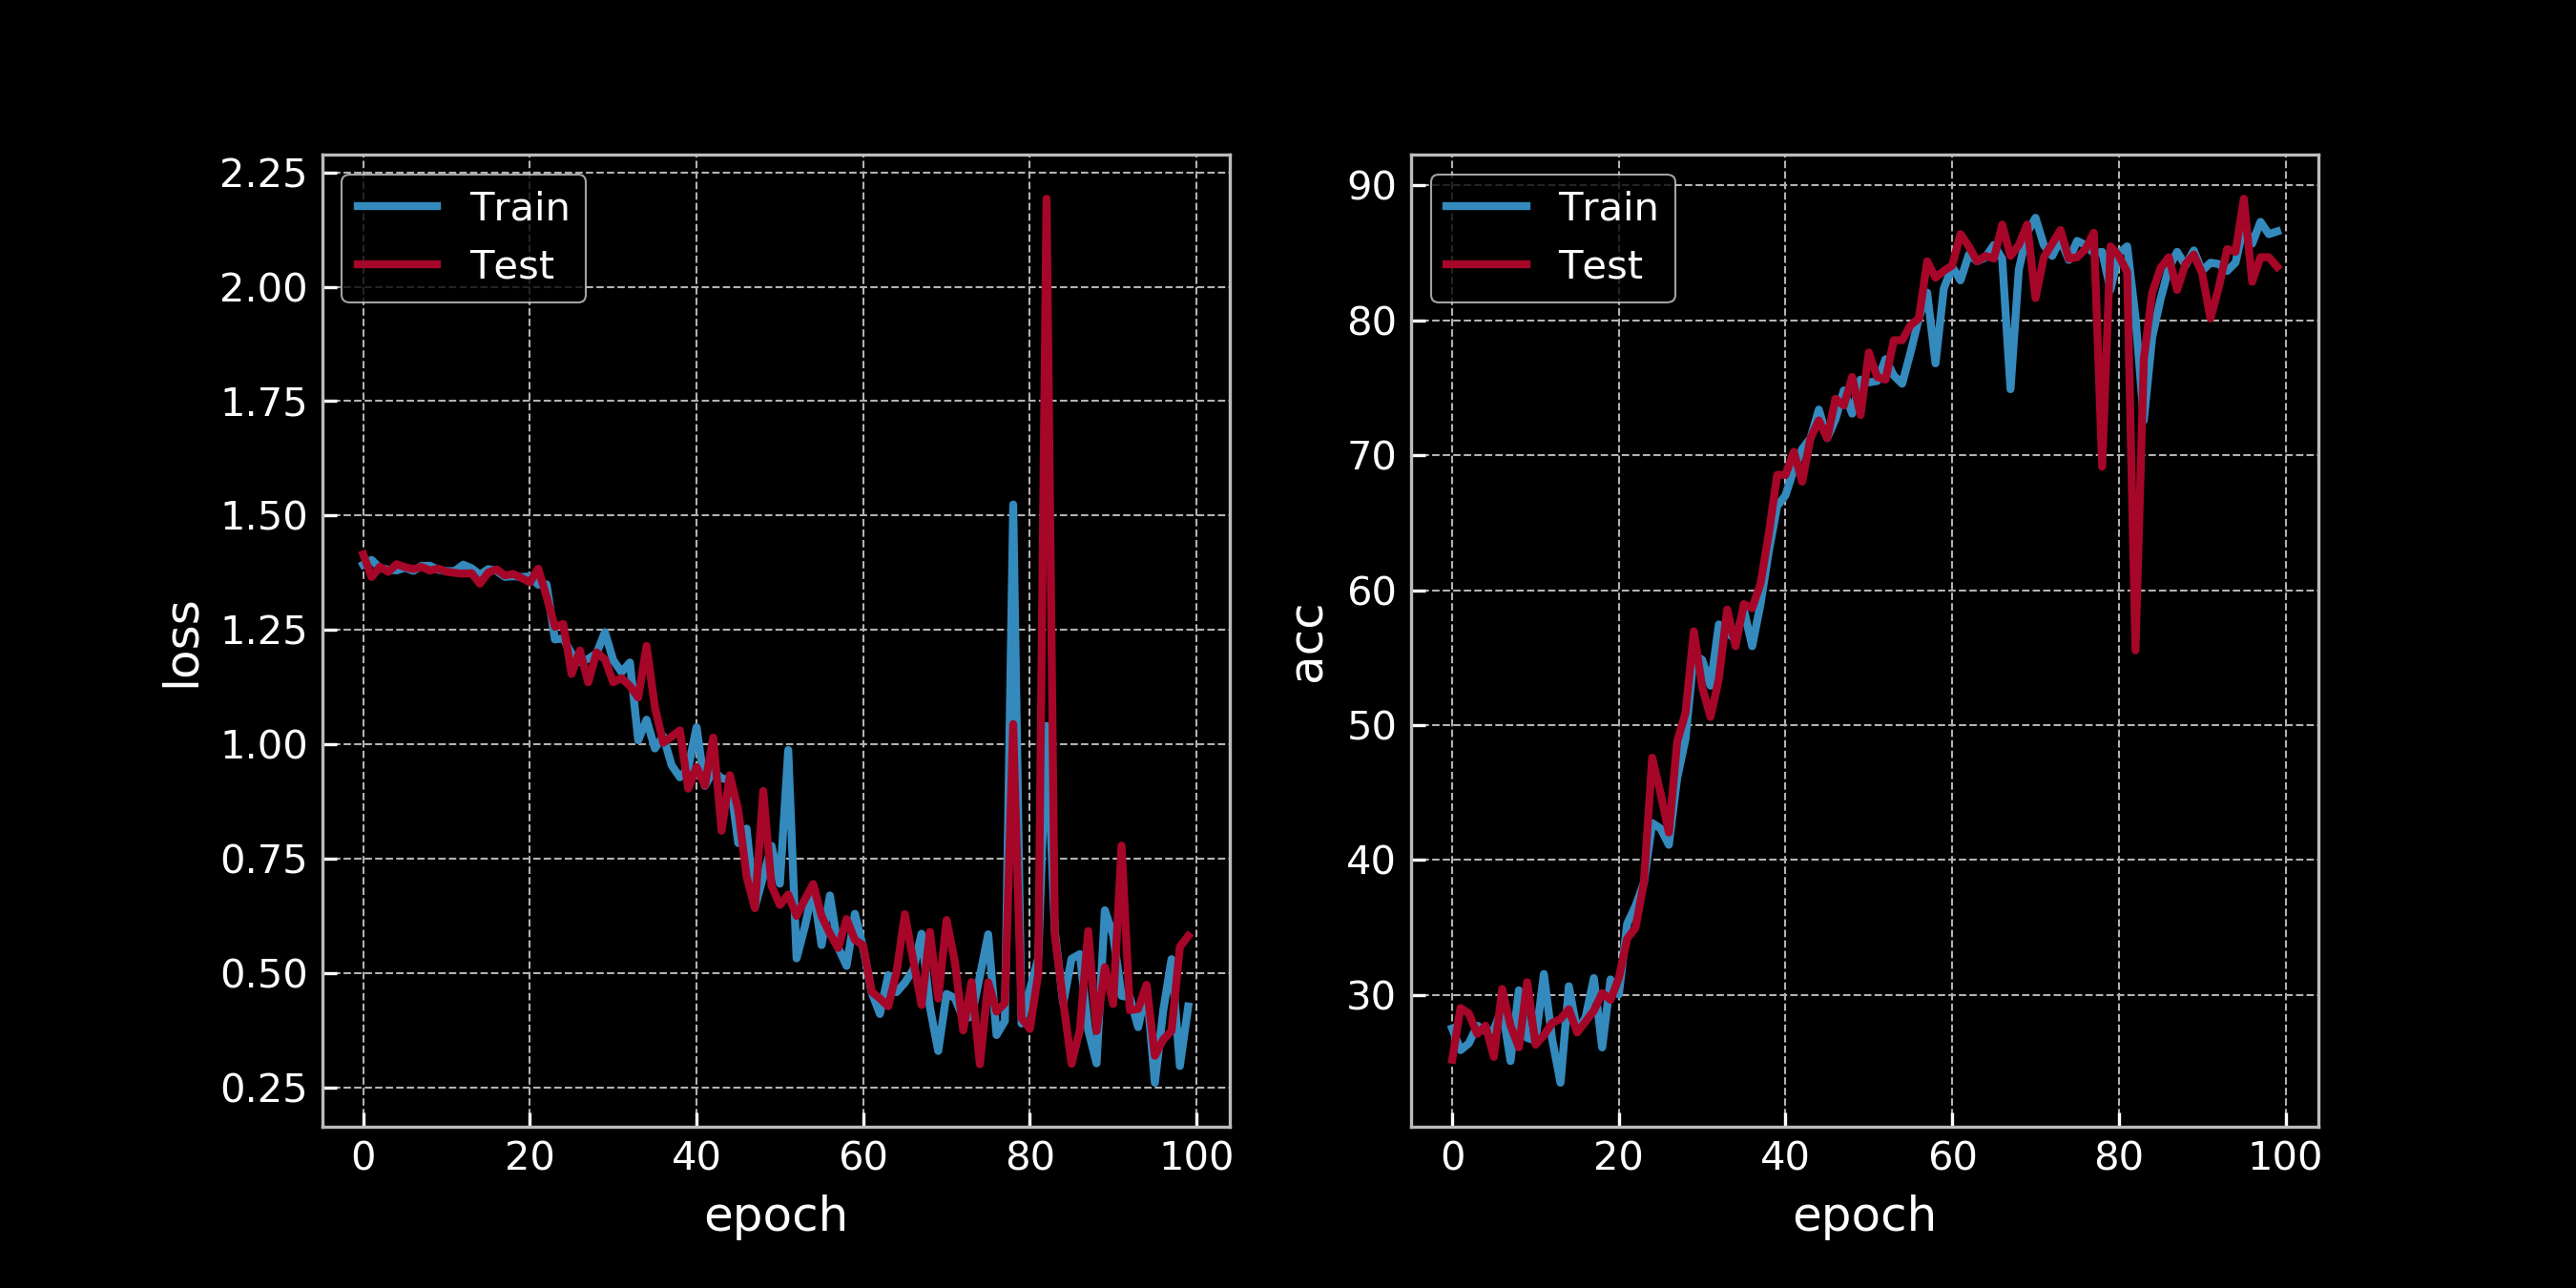
\includegraphics[width=0.5\linewidth]{labs/08/images/lstm_moderate_100.png}
    \caption{MODERATE Difficulty - LSTM Model for 100 epochs}
    \label{fig:lstm_moderate_100}
\end{figure}

The RNN model performs poorly with a testing accuracy of $\approx 26\%$. 
This is equivalent to randomly predicting one of the classes.
The corresponding loss is $\approx 1.39$ which is around $-\ln(0.25)$ as expected.

In comparsion, the LSTM model still achieves accuracy $\approx 84\%$ and thus exhibits long-term memory.

Since LSTM has 4 times the parameters than RNN, this is not a fair comparison. 
Despite this fact, it sheds light on the ability of LSTM to maintain long-term memory.

\section{Signal Echoing}
In signal echoing, given an input sequence, the task is to regenerate the same sequence with a lag of $n$ steps. 
This is an example of synchronized many-to-many task as both input and output are sequences. 
The input is a random binary sequence. 
Full details about the implementation of this problem can be found at \href{https://github.com/Atcold/pytorch-Deep-Learning-Minicourse/blob/master/09-echo\_data.ipynb}{Echo Data}.

\subsection{Data Generation and exploration}
The data is generated using the \texttt{EchoData} class. A call to this class generates \texttt{x\_batch}, \texttt{y\_batch}, \texttt{x\_chunk} and \texttt{y\_chunk}.
\texttt{x\_batch} contains \texttt{batch\_size} number of sequences each of length \texttt{series\_length}. Thus it's shape is (\texttt{batch\_size}, \texttt{series\_length}).
\texttt{y\_batch} contains the same data as \texttt{x\_batch} but it is shifted towards right by \texttt{echo\_steps} number of steps. It is appended by zeros in the beginning to match the size of \texttt{x\_batch}. 
Let us visualize the batches with \texttt{batch\_size} = $5$ and \texttt{series\_length} = $20000$.

\begin{verbatim}
    x_batch:
0 0 1 0 0 1 0 0 1 0 1 0 0 0 0 1 0 1 1 1 ...
0 1 1 0 0 1 0 1 1 0 1 1 0 1 1 1 0 0 1 1 ...
1 0 0 1 0 0 0 1 1 0 0 1 0 0 1 0 1 1 1 1 ...
1 0 0 0 1 0 1 1 0 1 1 0 0 0 1 1 1 1 1 1 ...
1 0 0 0 1 1 0 1 1 1 0 0 1 0 1 1 0 0 1 1 ...
x_batch size: (5, 20000)

y_batch:
0 0 0 0 0 1 0 0 1 0 0 1 0 1 0 0 0 0 1 0 ...
0 0 0 0 1 1 0 0 1 0 1 1 0 1 1 0 1 1 1 0 ...
0 0 0 1 0 0 1 0 0 0 1 1 0 0 1 0 0 1 0 1 ...
0 0 0 1 0 0 0 1 0 1 1 0 1 1 0 0 0 1 1 1 ...
0 0 0 1 0 0 0 1 1 0 1 1 1 0 0 1 0 1 1 0 ...
y_batch size: (5, 20000)
\end{verbatim}
Since backpropagating through a series of length $20000$ is practically in feasible, we divide the series in chunks of length \texttt{truncated\_length}. 
The RNN is supplied these chunks as inputs sequentially.
Let us visualize one of the chunks.

\begin{verbatim}
    x_chunk:
[0 1 1 0 0 1 0 0 0 0 1 0 1 0 0 1 0 1 1 1]
[0 1 0 0 0 0 1 1 0 0 0 1 1 1 0 1 0 0 0 0]
[1 0 0 0 1 0 0 0 1 0 1 1 1 1 0 1 0 0 0 1]
[0 0 0 0 0 1 1 0 1 1 1 0 1 0 1 0 0 1 0 1]
[1 1 0 1 0 0 0 1 1 1 0 0 0 1 0 0 1 1 0 1]
1st x_chunk size: (5, 20, 1)

y_chunk:
[1 1 1 0 0 0 0 1 0 1 1 0 0 1 0 0 0 0 0 0]
[0 0 0 1 0 1 1 1 1 1 1 0 1 0 1 0 0 0 0 1]
[0 0 1 1 1 1 1 0 0 0 1 0 1 1 0 1 0 1 0 0]
[1 0 1 0 0 1 0 0 1 0 0 0 0 1 1 1 0 1 0 1]
[1 0 1 1 1 0 0 0 1 1 0 0 0 0 0 0 1 1 0 1]
1st y_chunk size: (5, 20, 1)
\end{verbatim}
Note that $1$ is appended to the dimension of the chunks because \texttt{torch.nn.RNN} assumes the input to be three dimensional where $3^{\text{rd}}$ dimension contains the input dimension which is 1 in our case (since we have binary sequence).

\subsection{Model Architecture}
The following class contains the architecture of the model -
\begin{minted}[breaklines]{python}
class SimpleRNN(nn.Module):
    def __init__(self, input_size, rnn_hidden_size, output_size):
        super().__init__()
        self.rnn_hidden_size = rnn_hidden_size
        self.rnn = torch.nn.RNN(
            input_size=input_size,
            hidden_size=rnn_hidden_size,
            num_layers=1,
            nonlinearity='relu',
            batch_first=True
        )
        self.linear = torch.nn.Linear(
            in_features=rnn_hidden_size,
            out_features=1
        )

    def forward(self, x, hidden):
        x, hidden = self.rnn(x, hidden)  
        x = self.linear(x)
        return x, hidden
\end{minted}
The model architecture is pretty straight forward. 
The input chunk is inputted in the RNN with 1 hidden layer. 
\texttt{batch\_first} set to True which makes the batch size as the first dimension for both input and output. 
RNN outputs a hidden vector and an output vector. The output vector is of shape (\texttt{batch}, \texttt{seq\_len}, \texttt{hidden\_size}). 
Since the output of the model have to be either 0 or 1, a linear layer is used to map the output of RNN from \texttt{hidden\_size} to a 2 dimensional space.

\subsection{Training}
The model is trained for 5 epochs using the training function shown below.
\begin{minted}[breaklines]{python}
def train(hidden):
    model.train()
       
    correct = 0
    for batch_idx in range(train_size):
        data, target = train_data[batch_idx]
        data, target = torch.from_numpy(data).float().to(device), torch.from_numpy(target).float().to(device)
        optimizer.zero_grad()
        if hidden is not None: hidden.detach_()
        logits, hidden = model(data, hidden)
        loss = criterion(logits, target)
        loss.backward()
        optimizer.step()
        
        pred = (torch.sigmoid(logits) > 0.5)
        correct += (pred == target.byte()).int().sum().item()
        
    return correct, loss.item(), hidden
\end{minted}
The important thing to note is the use of \texttt{hidden.detach\_()}.
It is necessary to use this as we are reusing the hidden states obtained from one chunk into another chunk. 
But we want the gradients to be back-propagated only over the sequences in the current chunk and not all the way back. \texttt{hidden.detach\_()} removes the hidden variable from computation graph and prevents the gradients to back-propagate through the variable.

The loss function used is \texttt{BCEWithLogitsLoss}. 
This loss combines a Sigmoid layer and the BCELoss in one single class where BCELoss measures the Binary Cross Entropy between the target and the output. 
This is more numerically stable than using a Sigmoid followed by a BCELoss as we take advantage of the log-sum-exp trick for numerical stability.

The model achieves training and test accuracy of 100\% after 5 epochs.

\subsection{Output Visualization}
The trained model is used to echo a random sequence. 
The output is shown below.
\begin{minted}[breaklines]{python}
# Let's try some echoing
my_input = torch.empty(1, 100, 1).random_(2).to(device)
hidden = None
my_out, _ = model(my_input, hidden)
print(my_input.view(1, -1).byte(), (my_out > 0).view(1, -1), sep='\n')
\end{minted}
\begin{verbatim}
    tensor([[1, 1, 0, 1, 1, 0, 1, 1, 1, 0, 1, 0, 1, 0, 1, 1, 1, 1, 1, 1, 0, 0, 1, 1,
         0, 0, 0, 1, 1, 0, 0, 0, 0, 0, 1, 1, 1, 1, 1, 1, 1, 0, 0, 1, 0, 0, 0, 1,
         0, 1, 0, 1, 0, 0, 0, 0, 1, 1, 0, 0, 0, 1, 0, 1, 1, 0, 0, 1, 0, 1, 0, 0,
         0, 1, 0, 1, 0, 1, 1, 1, 0, 1, 0, 1, 1, 1, 1, 0, 0, 1, 0, 0, 0, 0, 1, 1,
         0, 1, 1, 0]], dtype=torch.uint8)
tensor([[0, 0, 0, 0, 1, 0, 1, 1, 0, 1, 1, 1, 0, 1, 0, 1, 0, 1, 1, 1, 1, 1, 1, 0,
         0, 1, 1, 0, 0, 0, 1, 1, 0, 0, 0, 0, 0, 1, 1, 1, 1, 1, 1, 1, 0, 0, 1, 0,
         0, 0, 1, 0, 1, 0, 1, 0, 0, 0, 0, 1, 1, 0, 0, 0, 1, 0, 1, 1, 0, 0, 1, 0,
         1, 0, 0, 0, 1, 0, 1, 0, 1, 1, 1, 0, 1, 0, 1, 1, 1, 1, 0, 0, 1, 0, 0, 0,
         0, 1, 1, 0]], dtype=torch.uint8)
\end{verbatim}
The model successfully echoes the data after 3 steps except the start of the sequence. 
This is because a None hidden state is supplied to the model and it takes some time to transform into a meaningful state.


